
% This is a modified version of the IEEE Latex template
% Author: Micah Flack 

\documentclass[conference]{IEEEtran}
\IEEEoverridecommandlockouts
% The preceding line is only needed to identify funding in the first footnote. If that is unneeded, please comment it out.
% \usepackage{cite}
\usepackage{amsmath,amssymb,amsfonts}
\usepackage{algorithmic}
\usepackage{graphicx}
\usepackage{textcomp}
\usepackage[table]{xcolor} % for cell colors
\usepackage{tabularx}
\usepackage{float}


% Bibliography settings

\def\BibTeX{{\rm B\kern-.05em{\sc i\kern-.025em b}\kern-.08em
    T\kern-.1667em\lower.7ex\hbox{E}\kern-.125emX}}


% not using numeric-comp, latex will default to [1], [2] instead of [1,2].
\usepackage[backend=biber, style=ieee, citestyle=numeric-comp]{biblatex} % ieee citation style

% Bibliographies... auto-updated w/ Zotero

\addbibresource{Main.bib}
\addbibresource{Extra.bib}

\begin{document}

% Title pages

\title{PRINTSHOP: ASSESSING OS AND CAPABILITIES OF SERIAL PRINT DEVICES}

\author{\IEEEauthorblockN{1\textsuperscript{st} Micah Flack}
\IEEEauthorblockA{\textit{The Beacom College of Computer and Cyber Sciences} \\
\textit{Dakota State University}\\
Idaho Falls, USA \\
micah.flack@trojans.dsu.edu}
}

\maketitle

% Add each of the sections

\begin{abstract}
(OUTLINE FILLER WORDS) pharetra sit amet aliquam id diam maecenas ultricies mi eget mauris pharetra et ultrices neque ornare aenean euismod elementum nisi quis eleifend quam adipiscing vitae proin sagittis nisl rhoncus mattis rhoncus urna neque viverra justo nec ultrices dui sapien eget mi proin sed libero enim sed faucibus turpis in eu mi bibendum neque egestas congue quisque egestas diam in arcu cursus euismod quis viverra nibh cras pulvinar mattis nunc sed blandit libero volutpat sed cras ornare arcu dui vivamus arcu felis bibendum ut tristique et egestas quis ipsum suspendisse ultrices gravida dictum fusce ut placerat orci nulla pellentesque dignissim enim.
(OUTLINE FILLER WORDS).
\end{abstract}

\begin{IEEEkeywords}
serial devices, thermal printer, PoS, ICS, badusb, hardware hacking, embedded devices. 
\end{IEEEkeywords}

\chapter{\leavevmode Introduction}
\label{chap:introduction}

% \section*{Overview}
% \addcontentsline{toc}{section}{Overview}
\section{Background}  \label{background}

Serial printers are devices commonly used for instant reporting of system data for industrial control systems (ICS) and receipts for point-of-sale (POS) systems. These devices are connected to their host using Wi-Fi, bluetooth, ethernet, or USB; in some cases, serial RS232 is an option as well. The goal of this research is to assess what software and hardware protections are enabled, as well as, how configurable the serial printers are for further exploit research.


\begin{figure}[ht]%
  \centering
  \subfloat[\centering Square POS]{{ 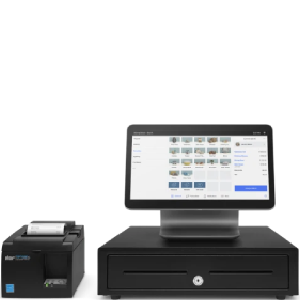
\includegraphics[width=0.30\textwidth,keepaspectratio]{Figures/MidSquare.png} }}%
  \qquad
  \subfloat[\centering SurePOS]{{ 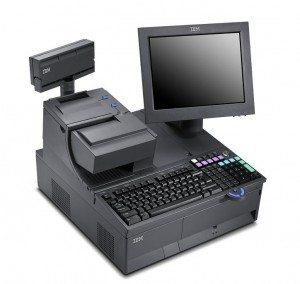
\includegraphics[width=0.25\textwidth,keepaspectratio]{Figures/SurePOS.jpg} }}%
  \caption{Comparison of common POS systems}%
  \label{fig:comparison_pos}%
\end{figure}

Figure \ref{fig:comparison_pos} shows us two similar looking point-of-sale systems. However, the operating system and required hardware used by both is different. Typically, unless you have the Square provided terminal, their software/client is installed onto an Android or iOS device and connected to a Square compatible card reader \autocite{ondrusMobilePaymentsMarket2011}. Whereas, the SurePoS, NCR, or other common EFTPoS system will run a proprietary OS based on Windows or Linux \autocite{ebimoboweiROLESOFTWARECASHLESS2018}. Furthermore, these PoS require some form of printing receipts as record keeping for the business owner and customer. And these devices also vary in terms of processing capabilities and operating system.

For instance, a common thermal printer seen with PoS systems, integrated with fuel pumps, or other industrial control equipment, is the SNBC BTP-S80 thermal printer \autocite{SNBCBTPS80Thermala,SNBCNewBeiyangIntelligent}. There are multiple versions of the device with support for Bluetooth, USB only, or combination of USB/Serial/Ethernet. The bluetooth hardware is provided over an accessory 25-pin serial connection, with more I/O as a serial connection via RS232C connector and USB Type-B. It has driver support for various platforms: Android, iOS, Windows, Linux, and MacOS. The most interesting aspects are the processor, an Arm Cortex M4 clocked at 3.54MHz, and the operating system, a proprietary version of FreeRTOS. The system architecture is Armv7E-M with JTAG/SWD hardware debugging support \autocite{CortexM4,FreeRTOSMarketLeading}.

By default, the printer has enough headroom to process ESC/POS commands for printing paper and a webserver for debugging or general diagnostics. In theory, the uncompromised device could be flashed with modified firmware to act as a decoy and human-input-device (HID) against the host PoS. The viability of any vulnerabilities would likely be dependent upon supply chain attacks or physical bait-and-switch tactics \autocite{scaifeFearReaperCharacterization2018}.

% In this paper, we propose exploring the processing capabilities and extensibility of FreeRTOS to act as a dual HID clone and printer for continued research.

\section{Significance}  \label{significance}

According to the Federal Trade Commission (FTC), there were 37,932 reports of credit card fraud in 2012 and 87,451 reports in 2022 \autocite{ConsumerSentinelNetwork2023,forthesentinelConsumerSentinelNetwork2022}. This marks an increase of credit card payment fraud by an estimated, 30.5\%. By comparison, since 2020, there has been a 14.6\% increase in credit card related fraud. Which does not include the millions of other fraud reports the FTC receives every year. In 2022 alone, there were around 5.1 million fraud, identity theft, and miscellaneous reports in total \autocite{ConsumerSentinelNetwork2023,forthesentinelConsumerSentinelNetwork2022}. The statistics for these reports stresses how crucial the security of payment systems are, both physical and online. And, the need to secure them grows every year.

Spyduino is \autocite{karystinosSpyduinoArduinoHID2019} a working example of a programmable BadUSB device using an Arduino to mimic a Human Interface Device (HID). Arduinos are typically more accessible and easily developed compared to an embedded device whose design is more single purpose \autocite{griffithsECIAIR2019European2019,patnaikpatnaikuniComparativeStudyArduino2017}. Especially if the goal is to not modify hardware or require hands-on access for exploitation. However, the research shows us that is it possible create HID clones from scratch if the hardware is compatible.

The Arduino used in their research is powered by an ATmega328P microcontroller with 32KB flash memory, 2KB SRAM, and 1KB EEPROM. Compared to the most likely target device of our proposed research, the SNBC BTP-S80, it features an ARM Cortex M4 microcontroller with 512KB flash memory, 96KB SRAM, 4KB of EEPROM. This is relevant to the proposed research, because it shows that a device with similar hardware specifications was feasible; meaning, it is likely that our own research will be successful. BadUSBs are a known and tested area of research. The novelty of this proposal comes from the assessment of the printer devices and showing whether one could be used maliciously within their environments (e.g., PoS systems, or ICS).

\section{Research Goals and Objectives}  \label{researchgoalsobjectives}

This research primarily focuses on physical POS systems or terminals and their hardware (serial accessories), rather than online solutions. For instance, not mobile payment apps like Venmo, CashApp, Zelle, or Paypal \autocite{wangMobilePaymentSecurity2016} since their environments typically do not use serial print devices. It is also likely that more research would be needed for emulating touch inputs for mobile environments versus the traditional keyboard attacks that will be implemented. Presumably, the host-to-guest communication will not differ greatly
between other environments (e.g., ICS). If the printers have demonstrable weaknesses with an Ubuntu host, that will fulfill the testing requirements.

The goal of this research is to further establish academic works in regards to embedded printer devices testing and security. This area is loosely documented within academia and only mentioned vaguely in relation to statistical reports or applied research using entirely different environments. For instance, most researchers limit their analysis of the environment to smartphones and the corresponding payment app, or detection systems for card skimmers \autocite{scaifeFearReaperCharacterization2018}.

Through this research we hope to identify supply chain risks using side channel attacks from auxiliary devices. Some examples of how the research could be applied in the future vary: BadUSB/BashBunny \autocite{hak5BashBunny}, JuiceShop \autocite{OWASPJuiceShop}, DVWA \autocite{woodDAMNVULNERABLEWEB2023}, or Webgoat \autocite{OWASPWebGoatOWASP}. Works within the PoS system context or embedded systems discussing supply chain attacks through third-party hardware are limited.

% \section{Printers}  \label{printers}

% \begin{figure}[ht]%
%   \centering
%   \subfloat[\centering BTP-S80]{{ 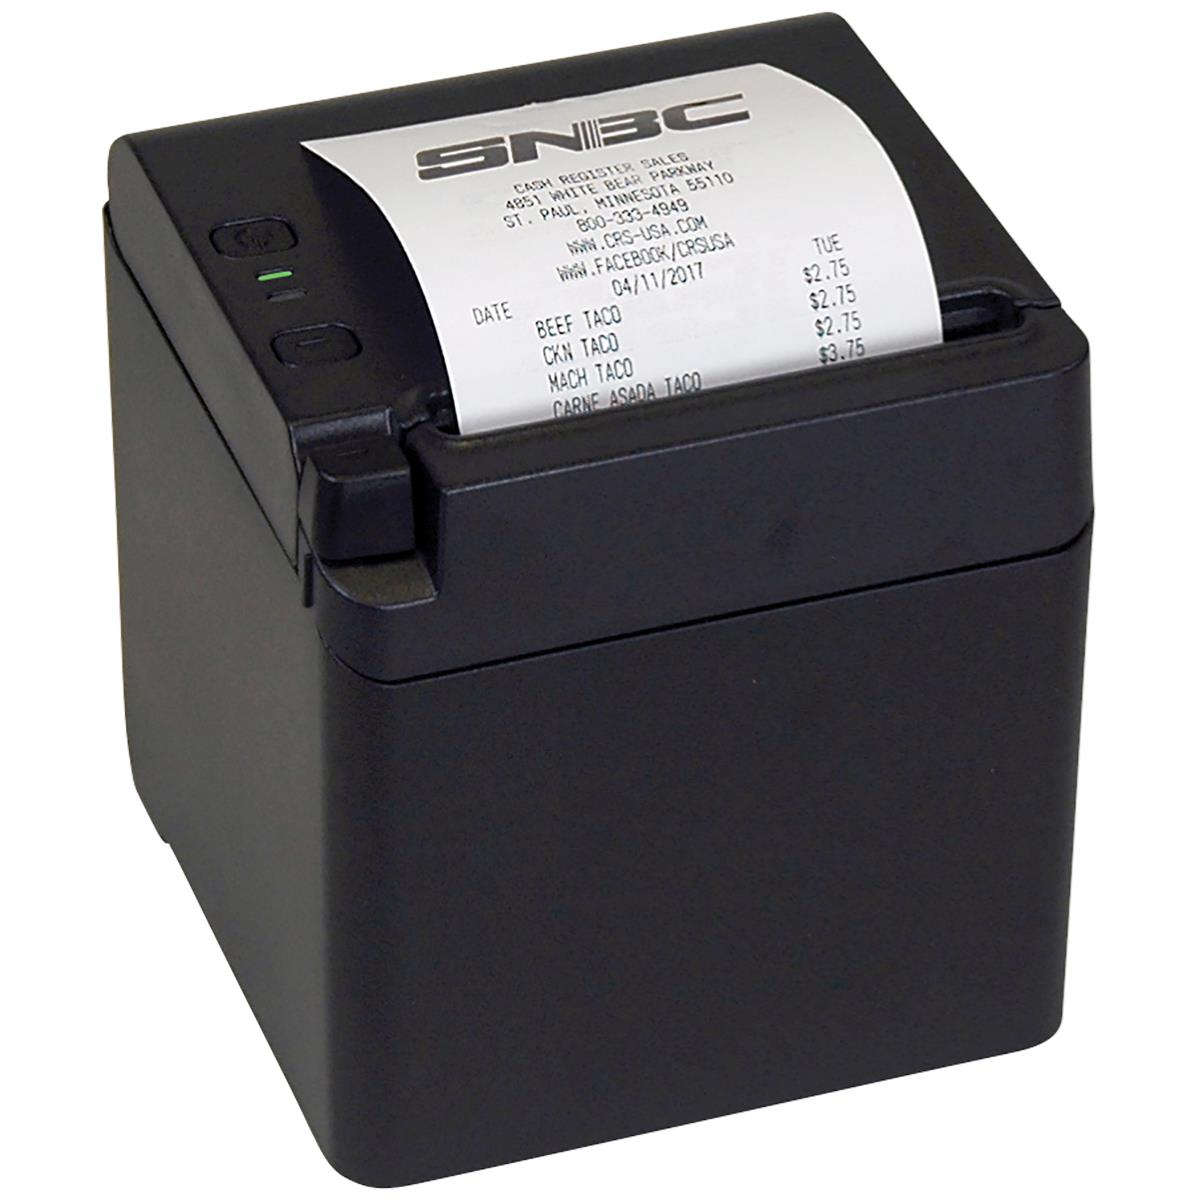
\includegraphics[width=0.40\textwidth,keepaspectratio]{Figures/SNBC_S80.jpeg} }}%
%   \qquad
%   \subfloat[\centering Printer I/O]{{ 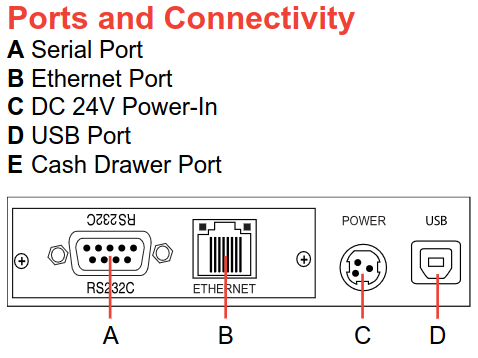
\includegraphics[width=0.40\textwidth,keepaspectratio]{Figures/SNBC_S80_IO.png} }}%
%   \caption{SNBC BTP-S80}%
%   \label{fig:btp_s80}%
% \end{figure}

% Figure \ref{fig:comparison_pos} shows us two similar looking point-of-sale systems, albeit one is much older looking. However, the operating system and required hardware is very different. Typically, unless you have the Square provided terminal, their software/client is installed onto an Android or iOS device and connected to a Square compatible card reader \autocite{ondrusMobilePaymentsMarket2011}. Whereas, the SurePoS, NCR, or other common EFTPoS system will run a proprietary OS derived from Windows or Linux \autocite{ebimoboweiROLESOFTWARECASHLESS2018}. Furthermore, these PoS tend to require some form of printing receipts as record keeping for the business owner and customer. And these devices also vary in terms of processing capabilities and operating system.

\section{Research Questions}  \label{researchquestions}

The research questions that this proposal seeks to answer are as follows:
\begin{itemize}
  \item Q1: Can the hardware be reflashed with a modified firmware image (e.g., FreeRTOS, ReconOS, VxWorks)? Testing a version of the original firmware with additional libraries, or an alternative OS, allows us to see if supply chain attacks are a concern. Either by the manufacturer, supplier, or other party. Reflashing is not novel by itself, however, the device might have protections in place to prevent it.  
  \item Q2: Does the hardware and firmware have enough resources to support HID functionality on-top of printing? In other words, can we maintain operation of standard printer command interpretation and side-channel input attacks without causing crashes or delays? The viability of the attack depends on it going unnoticed by operators or technicians. 
  \item Q3: Besides HID cloning, what other threat areas are exposed (e.g., network stack, web management portal, memory protections)? Are there any identifiable or known exploits when accessing the configuration panel (e.g., HTTP/2)? These provide a non-invasive method for bootstrapping the device.
\end{itemize}

Each of these goals will be approached individually as prescribed by the methodology.

\section*{Methodology}

There are several parts to the research methodology. First, technical information and datasheets were collected for each of the identified devices. Then, device capabilities were verified before beginning device teardown and flash recovery. During the disassembly, each component was documented and further technical information was gathered from respective manufacturers. The format for presenting the collected data is described later in section \ref{datacollectionprocess}.

\subsection{Research Approach} \label{researchapproach}

For this research, the quantitative approach and survey research was used \autocite{babbie2017basics,creswell2017research}. Because the goal of the research was to gather and examine, point-in-time, data across a sampled population of serial printer devices. By using quantitative survey research, it was possible to evaluate which devices are vulnerable to the attacks hypothesized, as well as, which devices are the most eligible for future design artifact research (i.e., creation of modified OS for HID cloning).


\subsection{Cross-Sectional Survey} \label{casestudy}

Using cross-sectional surveys \autocite{creswell2017research} has multiple benefits. It can be used to represent data as it is taken, rather than over a long period.  The study method also focuses on providing summaries that describe the patterns and context between collected data, and how it relates to the research questions.


\subsection{Data Collection Process} \label{datacollectionprocess}

The data collection process began with gathering technical specifications from device manufacturers. Typically, these contain information about the capabilities of the intended device functions. For a printer, this could contain information ranging from hardware specifications (e.g., CPU, architecture, memory) to things like printed pages per minute. This information forms the baseline for the device survey. Afterward, further specifications were gathered for components as each device was disassembled and examined. Roughly, the types and format of gathered device specifications appear as shown in Figure \ref{fig:device_specs} (e.g., SNBC BTP-S80 is used here).

\begin{table*}
  \centering
  \label{fig:device_specs}%
  \caption{Device specifications for SNBC BTP-S80}
  \begin{tabular}{|p{4cm}|p{12cm}|}
    \hline\rowcolor{gray!30}

    \textbf{Specifications} &  \\
    \hline

    Max print speed & 120mm (Two-Color), 150mm (Grayscale), 250mm (Mono) \\
    \hline

    Printing method & Direct Thermal \\
    \hline

    Paper roll type & 9 x 7, 82.5 x 80 x 57.5mm \\
    \hline

    Bar code support & UPC-A, UPC-E, EAN8, EAN13, Code39, Code93, CODE128, CODABAR, ITF, PDF417, QR Code, Maxicode \\
    \hline

    Printer interpreter & ESC/POS \\
    \hline

    Interfaces & Serial+USB+Ethernet \\
    &  USB+Parallel \\
    &  USB+Serial \\
    &  USB+Bluetooth \\
    &  USB+WiFi \\
    &  USB Only \\
    \hline

    Supported OS & 32-bit (Windows XP/2000/POSReady) \\
    &  64bit (Windows XP/Server 2012) \\
    &  32/64bit (Windows 10/8.1/8/7/Server 2008/Server 2003/Vista) \\
    &  Other (Linux/OPOS/BYJavaPOS Windows/BYJavaPOS Linux) \\
    \hline

    Development Kit & Android, iOS \\
    \hline

    Data Buffer & Receive Buffer RAM: 64KB \\
     &  RAM Bitmap: 128KB \\
     &  Flash Bitmap: 512KB \\
    \hline

    Power Supply & AC 100 $\sim$ 240V, 50/60 Hz Adapter \\
    \hline

    Current/Power Usage & 2.0A / 60W \\
    \hline

    Safety and EMI & FCC/UL \\
    \hline

  \end{tabular}
\end{table*}

Following the previous example, the next step in the data collection process would be identifying the SoC. If there is no beforehand knowledge, the SoC can be identified by comparing gathered datasheets during the components discovery. This is easily accomplished using an online service like FindChips or AllDataSheets \autocite{FindchipsElectronicPart}. The expected type and format for SoCs are described in Figure \ref{fig:soc_specs}.

The process for gathering flash/memory chip specifications was similar; identify the serial number and manufacturer, then find the component datasheet. Gathering the pin layouts and format is also useful for later stages, should the manual flash need to be recovered. The expected format for memory chips can be seen in Figure \ref{fig:memory_specs}.

\begin{table*}
  \centering
  \label{fig:soc_specs}%
  \caption{SoC technical specs example using Stellaris LM3S2793 Microcontroller}
  \begin{tabular}{|p{4cm}|p{12cm}|}
    \hline\rowcolor{gray!30}

    \textbf{Specifications} &  \\
    \hline

    Architecture & 32-bit ARM \\
    \hline

    Platform & ARM Cortex-M3 \\
    \hline

    Frequency & 80-MHz, 100DMIPS performance \\
    \hline

    Memory & 128KB single-cycle Flash memory \\
     & 64KB single-cycle SRAM \\
    \hline

    Firmware & Internal ROM loaded with StellarisWare \\
    \hline

    Advanced Comm. Interfaces & UART, SSI, I2C, I2S, CAN \\
    \hline

    Debug Interfaces & JTAG, SWD \\
    \hline

    Package format & 100-pin LQFP \\
    & 108-ball pin BGA \\
    \hline

  \end{tabular}
\end{table*}

\begin{table*}
  \centering
  \label{fig:memory_specs}%
  \caption{Memory specifications example using Infineon Technologies S25FL064P \autocite{S25FL064PSeriesFlash}}
  \begin{tabular}{|p{4cm}|p{12cm}|}
    \hline\rowcolor{gray!30}

    \textbf{Specifications} &  \\
    \hline

    Single power supply operation & 2.7 to 3.6V \\
    \hline

    Software Features & SPI Bus Compatible Serial Interface \\
    \hline

    Memory architecture & Uniform 64KB sectors \\
    & 256 byte page size \\
    \hline

    Programming & Page programming (up to 256 bytes) \\
    & Operations are page-by-page basis \\
    & Accelerated mode via 9V W\#/ACC pin \\
    & Quad page programming \\
    \hline

    Erase commands & Bulk erase function \\
     & Sector erase for 64KB sectors \\
     & Sub-sector erase for 4KB and 8KB sectors \\
    \hline

    Protections & W\#/ACC pin used with Status Register Bits to protect specified memory regions and configure parts as read-only; One time programmable area for permanent and secure identification \\
    \hline

    Package format & 16-pin SO \\
    & 8-contact WSON \\
    & 24-ball BGA, 5x5 pin config \\
    & 24 ball BGA, 6x6 pin config \\
    \hline

  \end{tabular}
\end{table*}

A final report will be created detailing each of these tables for the devices and their identified core components. Operating system features and protections will be loosely summarized for each device, there is no set reporting format or requirements. Using the final report will aid in the process of designing an artifact for future research and testing.

\subsection{Hardware Assessment} \label{hardwareassessment}

NIST SP 800-115 \autocite{NISTSP8001152020} provides general guidelines for performing information security testing and assessment, however, there is little information regarding hardware reverse engineering and firmware analysis. Their guidelines are aimed more towards single/multi-tasking operating systems like Windows or Unix-like, those where network logging and listener agents are feasible. For the targeted devices in this research proposal, a different approach is needed that evaluates the hardware protections of the SoC and flash memory. 

Analysis of device components, once disassembled, requires using a hardware debugger tool with the correct interface. The majority of the targeted devices use joint test action group (JTAG) or single wire debugging (SWD) headers. By referring to the manufacturer datasheet for a given SoC, it was possible to identify the pin layout for serial debugging access.

\begin{figure}[ht]%
  \centering
  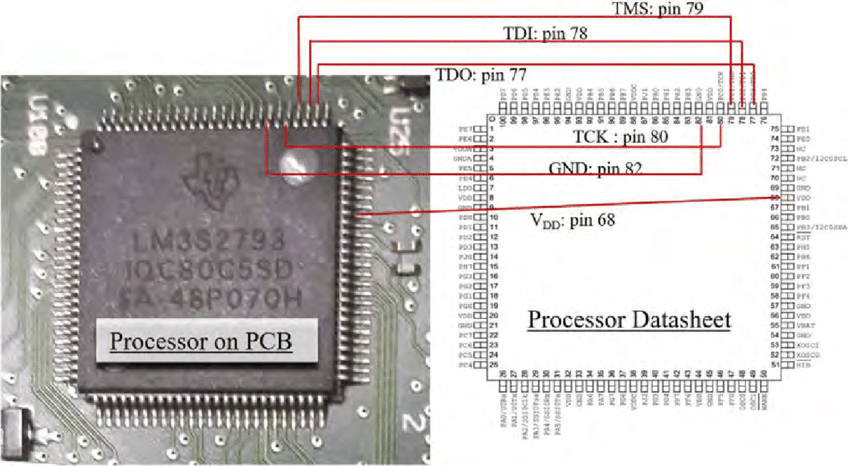
\includegraphics[keepaspectratio]{Figures/JTAGExample.png}
  \caption{JTAG pin out example for Texas Instruments LM3S2793}%
  \label{fig:jtag_pinout}%
\end{figure}

Figure \ref{fig:jtag_pinout} is an example showing what the physical SoC looks like on a PCB compared to the pin layout described in the datasheet. The dot in the top left of the SoC denotes the beginning of the pin layout. Counting in a counter-clockwise method indicates the pin number and the associated functions. For instance, to access the JTAG debug interface on the LM3S2793:

\begin{itemize}
  \item TDO: pin 77
  \item TDI: pin 78
  \item TMS: pin 79
  \item TCK: pin 80
  \item GND: pin 82
  \item V\textsubscript{DD}: pin 68
\end{itemize}

Using this information, a device like the JTAGULATOR \autocite{JTAGulator2023} can be connected and enumerate or verify pin layouts as described. Ball joint SoCs require a different process and are much harder to debug if there is no visible header available on the board. Once an interface is connected, if debugger access is not disabled, the researcher can interact with the bootloader to further investigate enabled protections and recover flash storage.

If the JTAG is disabled, the researcher would attempt to recover flash manually using a device like the Segger J-Link \autocite{SEGGERJLinkDebug}. The Segger has pre-defined and existing support for working with flash memory and flash breakpoints. Whereas, using OpenOCD with the JTAGULATOR would require time crafting custom configurations. Assuming there are no access protections to the flash memory, the researcher could begin performing firmware analysis to identify the operating system or potential vulnerabilities. Documenting the size and address range of memory regions was a key part of the process.

\section{Related Works}

\subsection{RTOS: Software and Security}
\autocite{Benadjila2018WooKeyU} introduces several embedded kernels and discusses their differences regarding developing a secure mass storage device. For this research, we are primarily interested in RTOS-like kernels because of existing support for a sample device like the SNBC BTP-S80 printer. However, the paper criticizes such operating systems because their "real-time driven design is largely incompatible with the overhead produced by security mechanisms." For many applications, there is a trade-off with RTOS where performance is the main criterion and security is not a priority. \autocite{yuRealTimeOperatingSystem} introduces several common RTOS and discusses their security issues. Notably, most RTOS are susceptible to code injection, cryptography inefficiency, unprotected shared memory, priority inversion, denial of service attacks, privilege escalation, and inter-process communication vulnerabilities. Depending on the MPU (microprocessor unit), the vendor has hardware protections like Intel SGX or Arm Trust Zone. These are all areas that can be used for pivoting onto the device, especially shared memory and privilege escalation. If the target device firmware is outdated (or, even libraries used by the firmware) and there are known CVEs that can be repeatedly exploited, persistence mechanisms are not a requirement to gain routine access.

\subsection{Embedded Firmware Patching}
Typically, updating the firmware for a device or even delivering patches requires a complete shutdown and hardware debug access (if supported). In some cases, the reflashing is unsupported through the operating system or bootloader and the flash memory needs to be reprogrammed. \autocite{heRapidPatchFirmwareHotpatching2022} describes a method for hot-patching downstream RTOS devices without needing to shut down or reboot. Any changes made are permanent and as effective as traditional delivery methods. RapidPatch was capable of patching over 90\% of vulnerabilities for the affected device, only needing at least 64KB or more memory and a 64 MHz MCU clock. This appears to be an effective method for attackers to sideload client or server implants without risking detection.

\subsection{BadUSB-like Devices}
BadUSB is a well-known and documented attack vector. One of the most popular hacker tools is built on the concept \autocite{hak5BashBunny}. However, there are some limitations:

\begin{itemize}
  \item Precision of attacks is limited since scripts or effects are typically deployed blind. There is no knowledge of the user environment nor ability to interact with functional user interface mechanisms (e.g., a mouse clicking a button). 
  \item Limited to the USB 2.0 standard. Meaning, no support for video adapters like HDMI, DisplayPort, or PowerDelivery like with USB 3.0. 
  \item There are existing methods for limiting USB access from the host, such as GoodUSB \autocite{tianDefendingMaliciousUSB2015}.
\end{itemize}

GoodUSB supports the Linux USB stack, so another solution would be required for Windows systems or RTOS. This all depends on the environment of the connected host, the PoS system. It is entirely possible that the PoS could have software like Crowdstrike Falcon deployed, which would monitor system behavior and mass storage device access \autocite{backer2021sdn}. Although the experiment environment will not use such software, it is an important distinction to make.

% Too much related works information... ?

% In \autocite*{tianSoKPlugPray2018}, they describe several attacks at each of the applicable layers to USB attacks: the human, application, transport, and physical layers. These attacks would typically require some human element for deployment, but that is not the focus of the research (e.g., social engineering versus hardware hacking). Whereas the physical layer could allow signal eavesdropping or injection. This could enable a modified printer to overvolt the host (USBKiller \autocite{USBKillDevices}) to cause physical damage or perform other side-channel attacks \autocite*{sridharEMIIssuesUniversal2003}. Either of those methods would require investigating the device hardware to determine what level of control the bootloader or operating system has over power delivery.


\section{Results}

Due to time constraints and under-budgeting, the actual sample size for this research is smaller than initially proposed. The original proposal estimated a small sample population of three to five of the most common, accessible serial printers. However, the shipment of additional printers would have taken longer than the submission deadline. All data presented is limited to available equipment at the time of reporting, the SNBC BTP-S80 serial printer.

\subsection{Device Disassembly} \label{devicedisassembly}

% \textbf{Outline}
% $\downarrow$

% \begin{itemize}
%     \item Walkthrough of documented teardown of the serial printer
%     \item Show pictures of each stage/device layers
%     \item Label pictures indicating functionality for regions of each layer (power deliver, data, I/O...)
%     \item Provide labeled key to refer in later sections
%     \item Could manufacturer increased physical security (?)
% \end{itemize}

% \textbf{The random ipsum lorem text is to gauge how much will be written when done. This will appear several times throughout the outline.}

The SNBC BTP-S80 is a common thermal printer used for providing receipts for PoS systems and immediate reporting for industrial control systems (ICS). This model features three buttons on the front face of the printer. Starting from the top: paper roll release, auto-feeding, and power button.  

\begin{figure}[ht]
    \centering
    {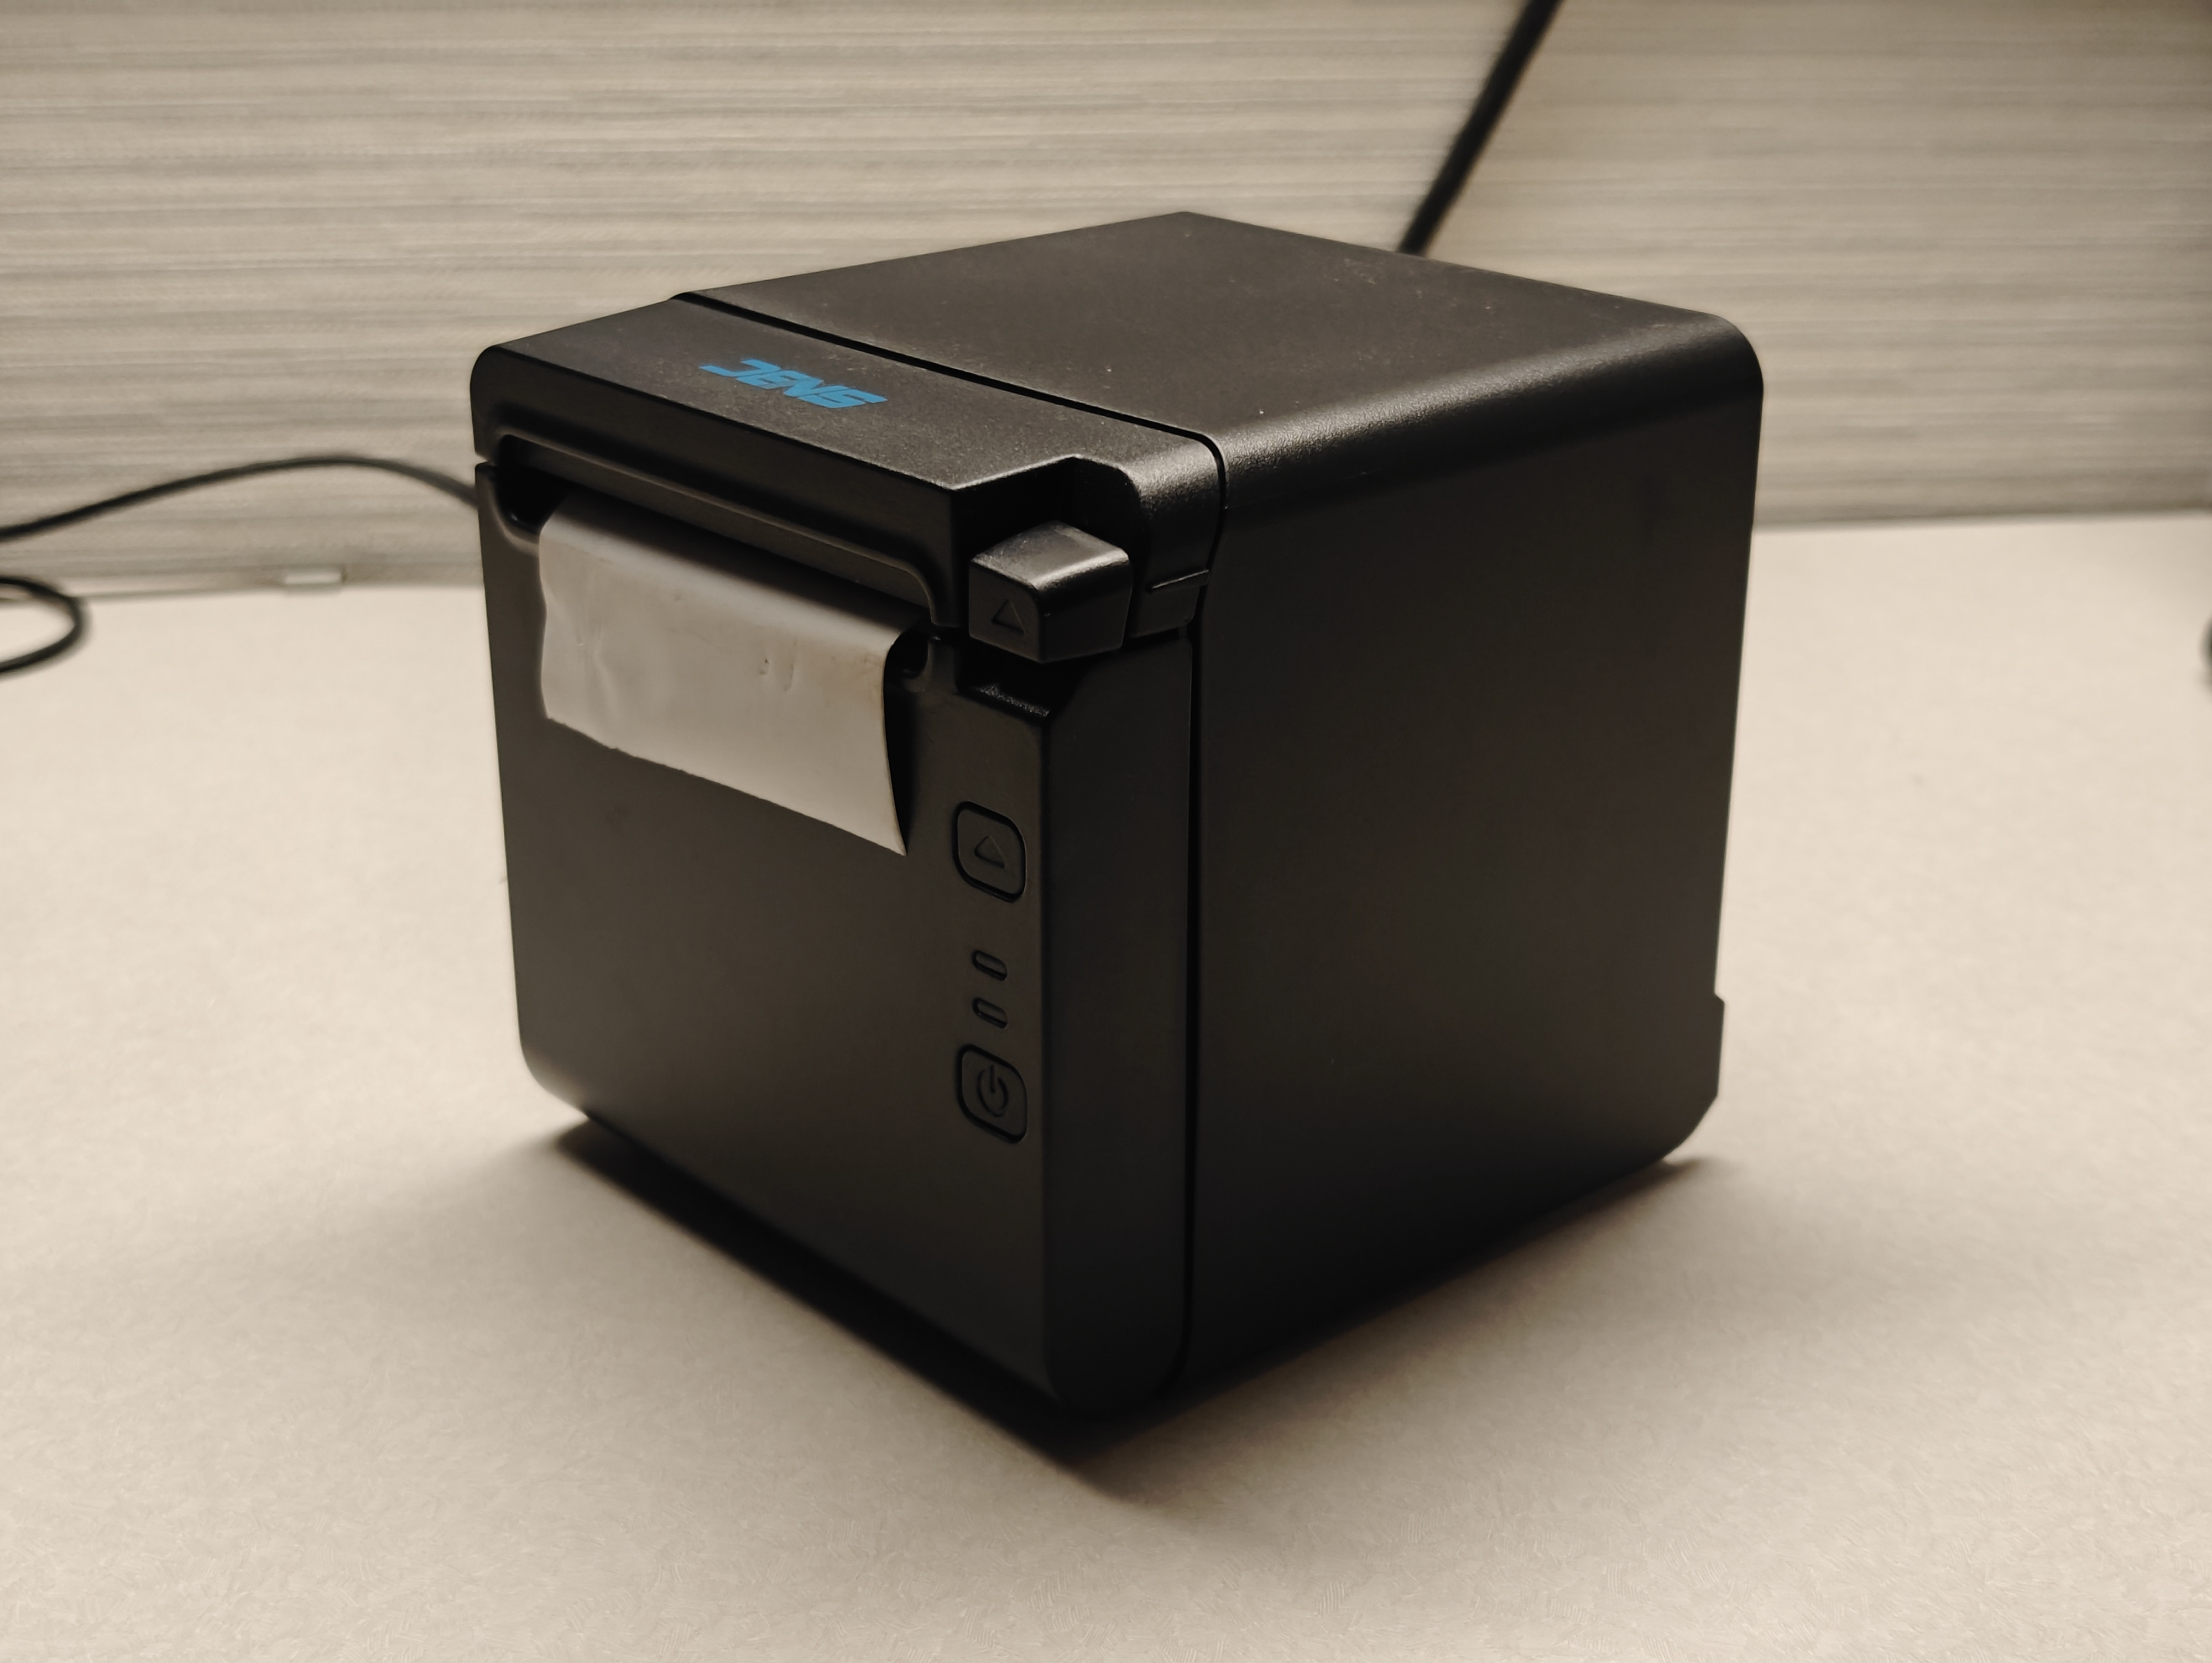
\includegraphics[width=88mm,scale=0.5]
    {Figures/Teardown/IMG20231204170511.jpg}}
    \caption{SNBC BTP-S80}
    \label{fig:snbc_btp_s80}
\end{figure}

From the rear of the device, we can see some of the available I/O. There are several ways to interface with the thermal printer. The host device can connect using an internet address via the RJ45 ethernet connector or over serial using the USB type-b and RS232. We can also see a screw on either side of the expansion card containing the RJ45 jack and RS232 connector. The manufactures website shows that this slot is interchangeable and can provide different functionality depending on the end-users needs. Some configurations are setup as shown in Figure \ref{fig:snbc_btp_s80_io}, others feature wireless adapters utilizing 2.4Ghz networking.

\begin{figure}[ht]
    \centering
    {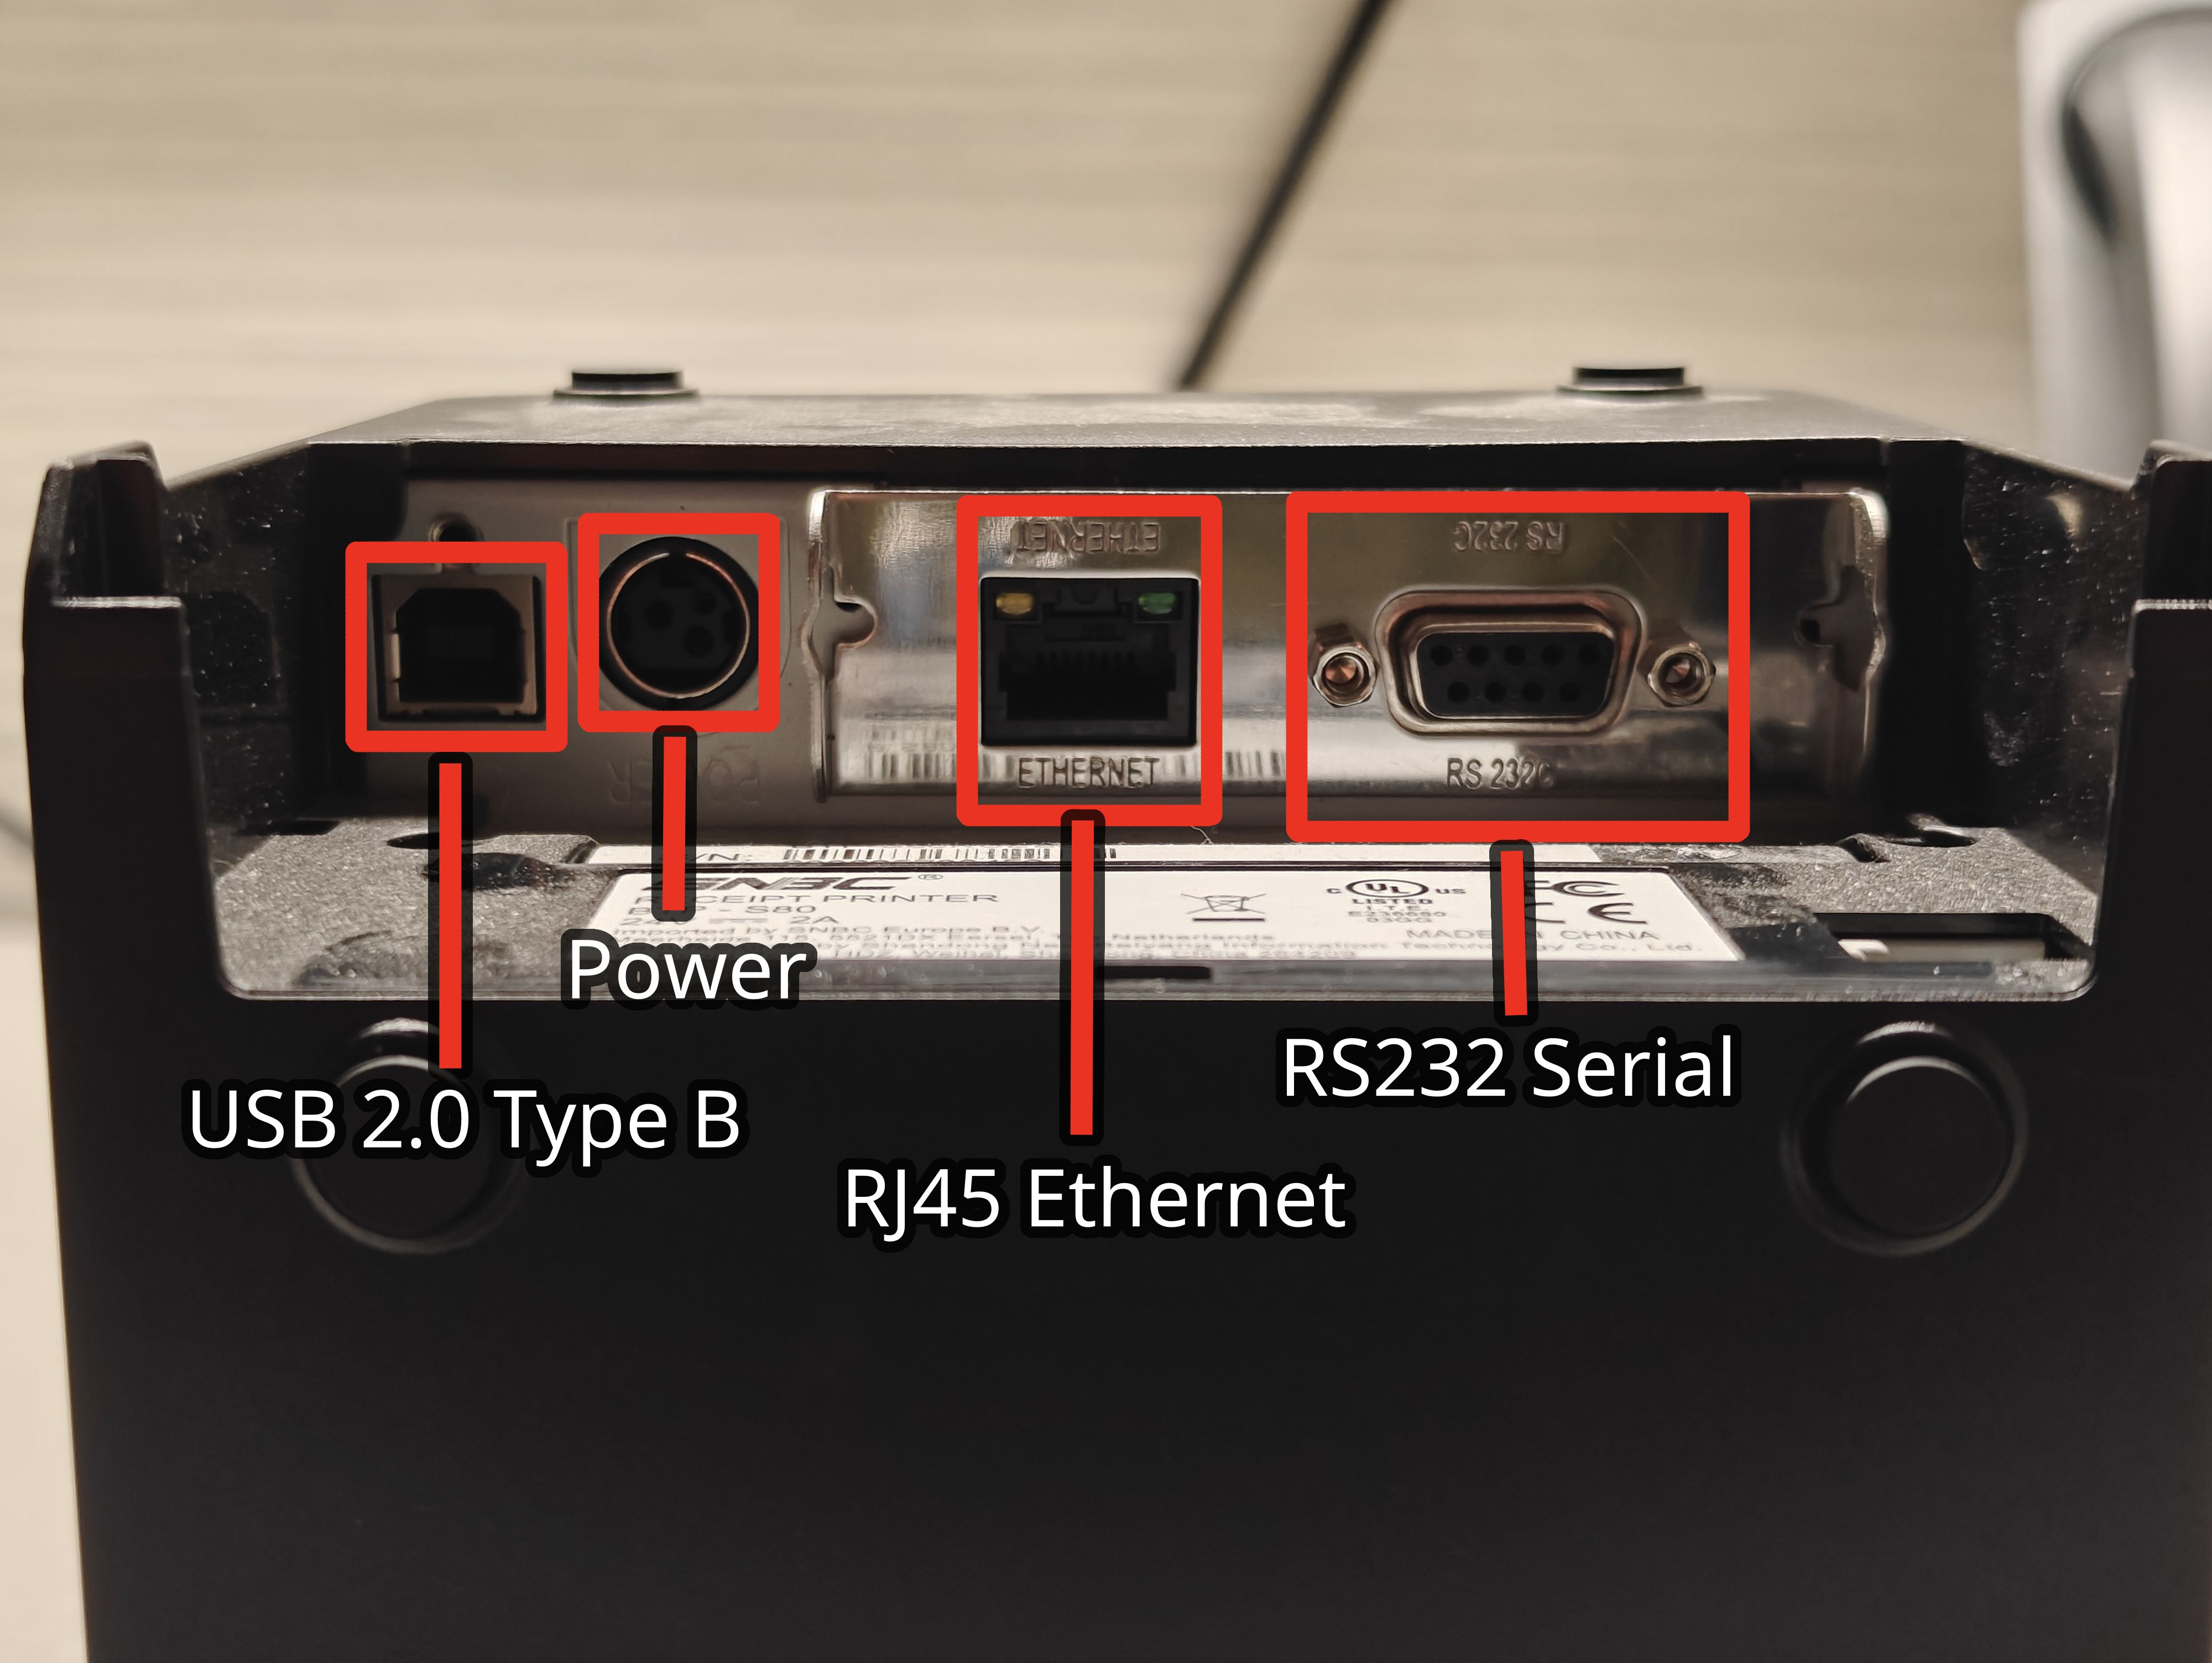
\includegraphics[width=88mm,scale=0.5]
    {Figures/Teardown/IMG20231204170442_annotated.jpg}}
    \caption{SNBC BTP-S80 labeled I/O}
    \label{fig:snbc_btp_s80_io}
\end{figure}

Removing each of the screws allows us to slide the chassis out of the outer shell. Here we can see the motherboard (leftmost) and the expansion cards (topside, right of the motherboard). The expansion cards are divided into two parts, as shown in Figure \ref{fig:snbc_btp_s80_expansion}.

\begin{figure}[ht]
    \centering
    {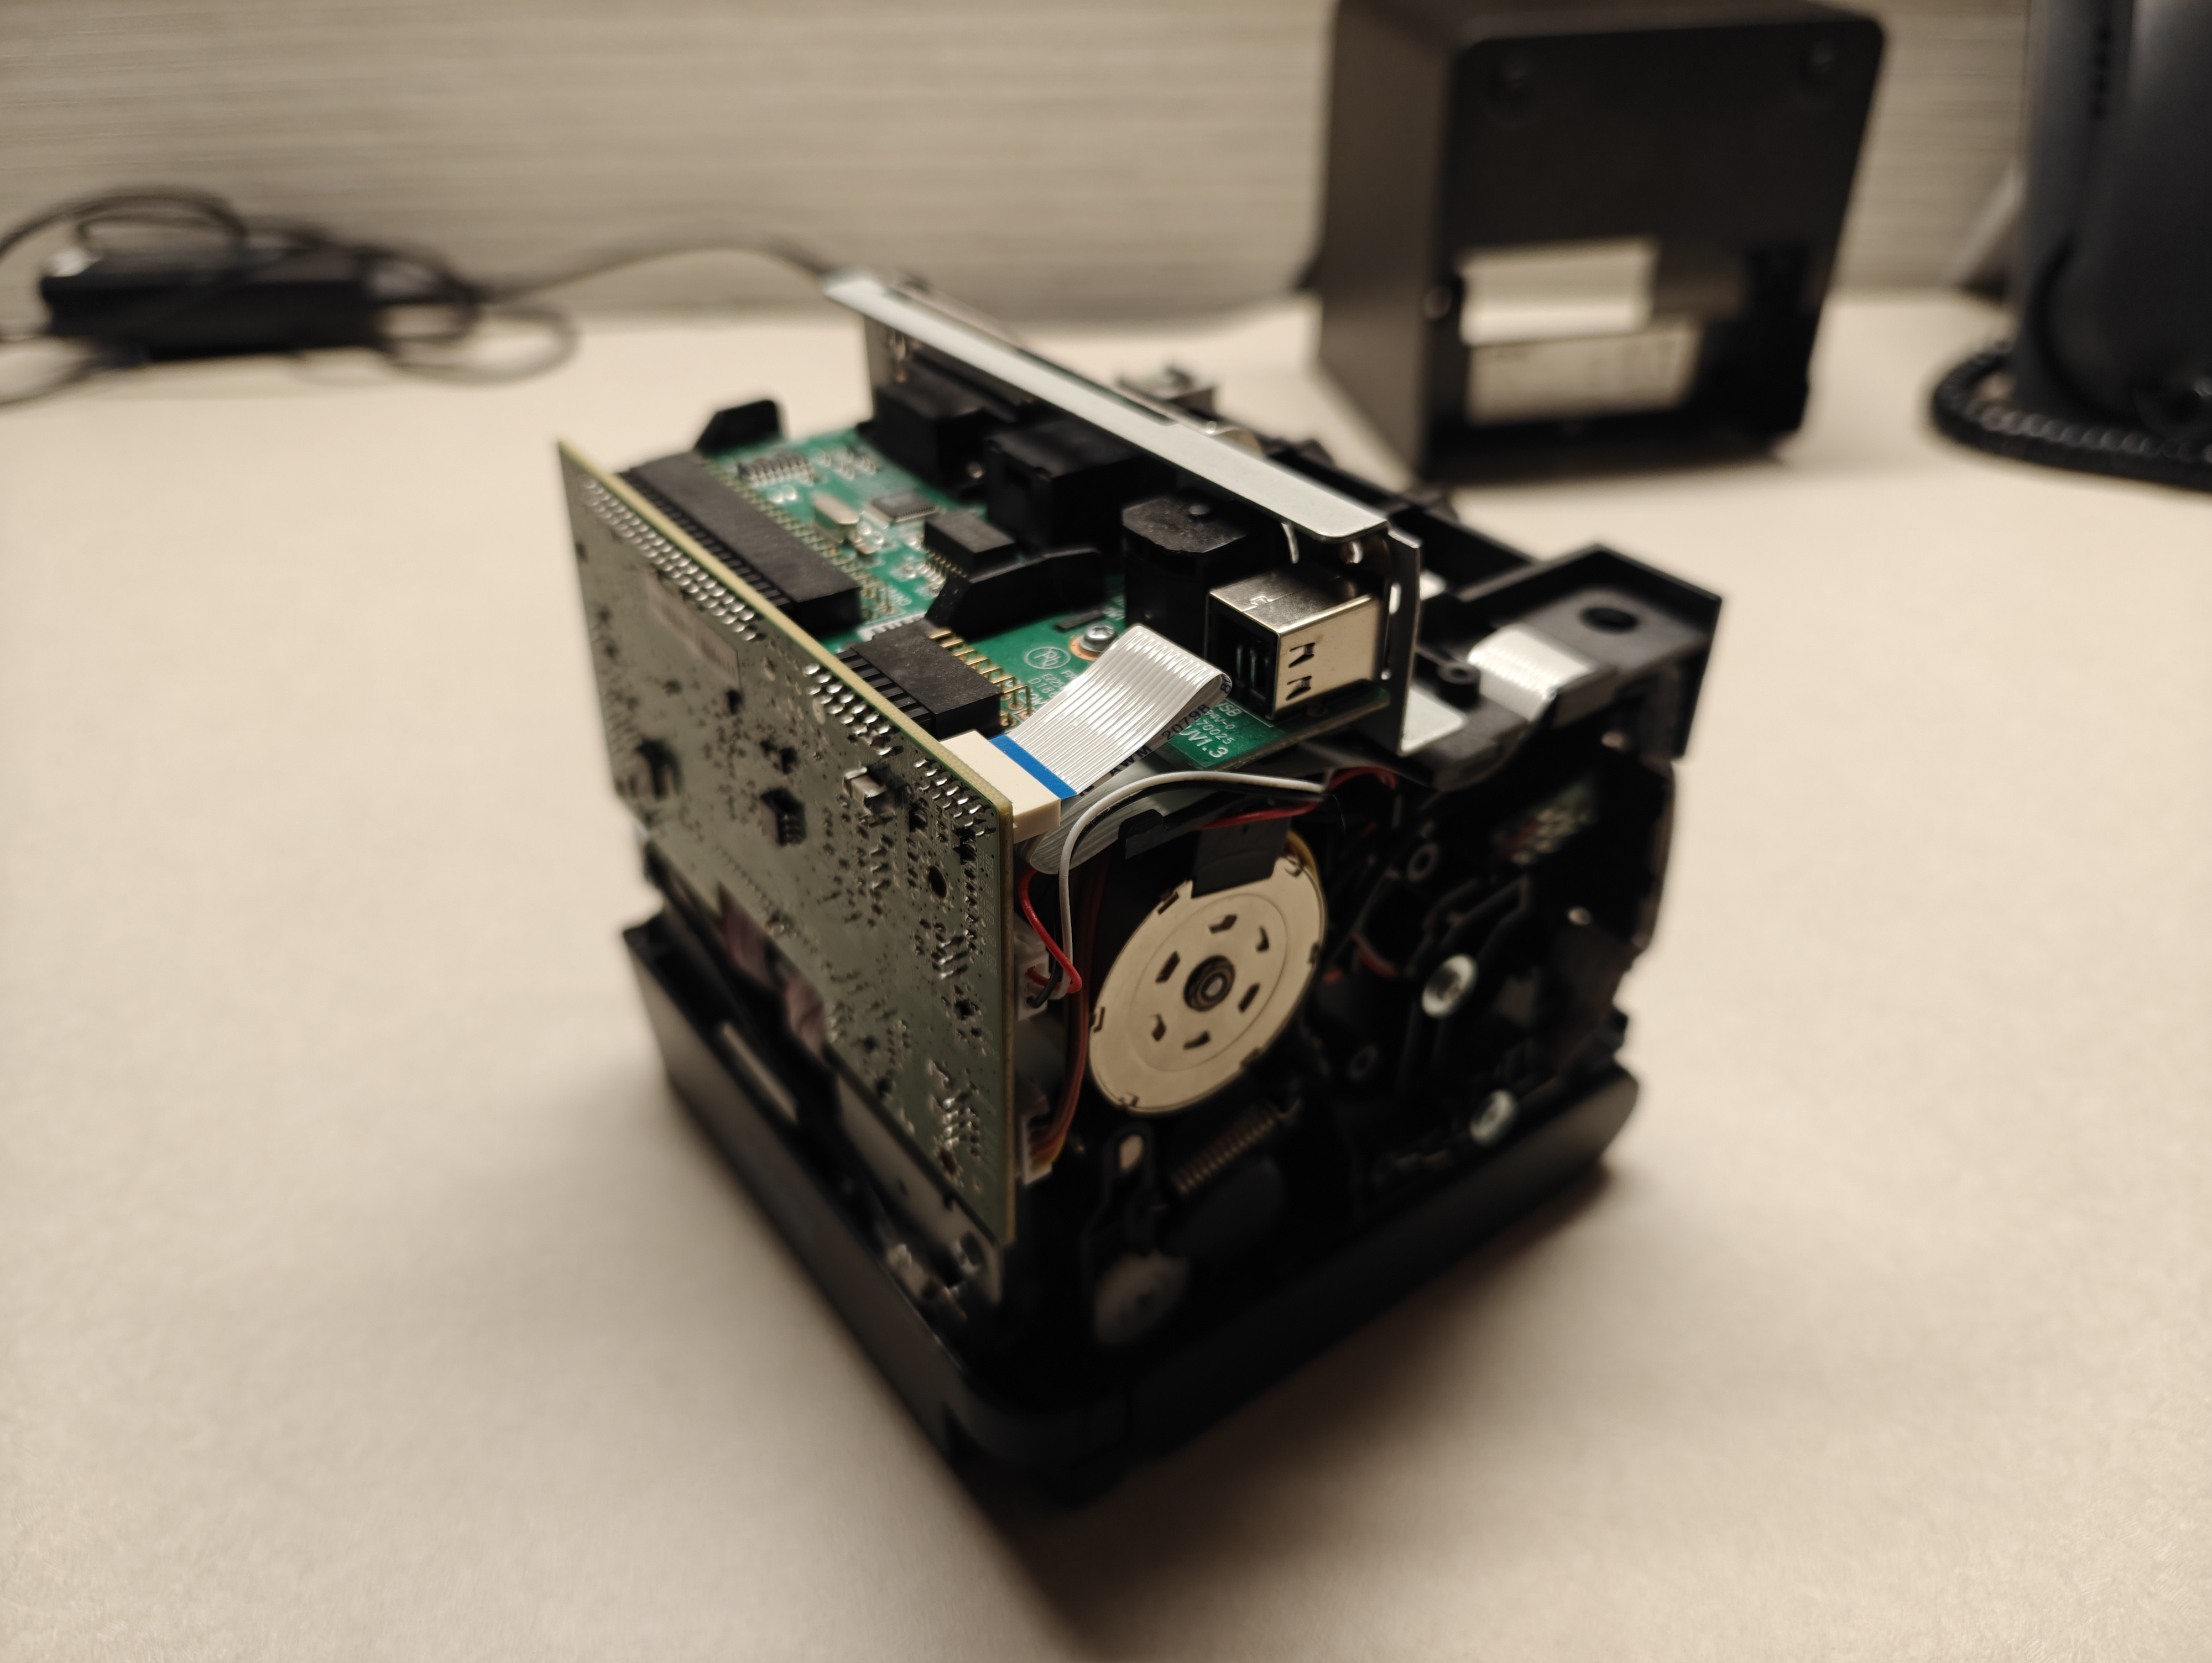
\includegraphics[width=88mm,scale=0.5]
    {Figures/Teardown/IMG20231204170938.jpg}}
    \caption{SNBC BTP-S80 inner chassis}
    \label{fig:snbc_btp_s80_chassis}
\end{figure}

The left expansion card allows the user of the device to swap networking stacks. In this configuration it features the RJ45 Ethernet and RS232 serial connector. The right expansion card provides USB connectivity and power via the barrel plug connector. 

\begin{figure}[ht]
    \centering
    {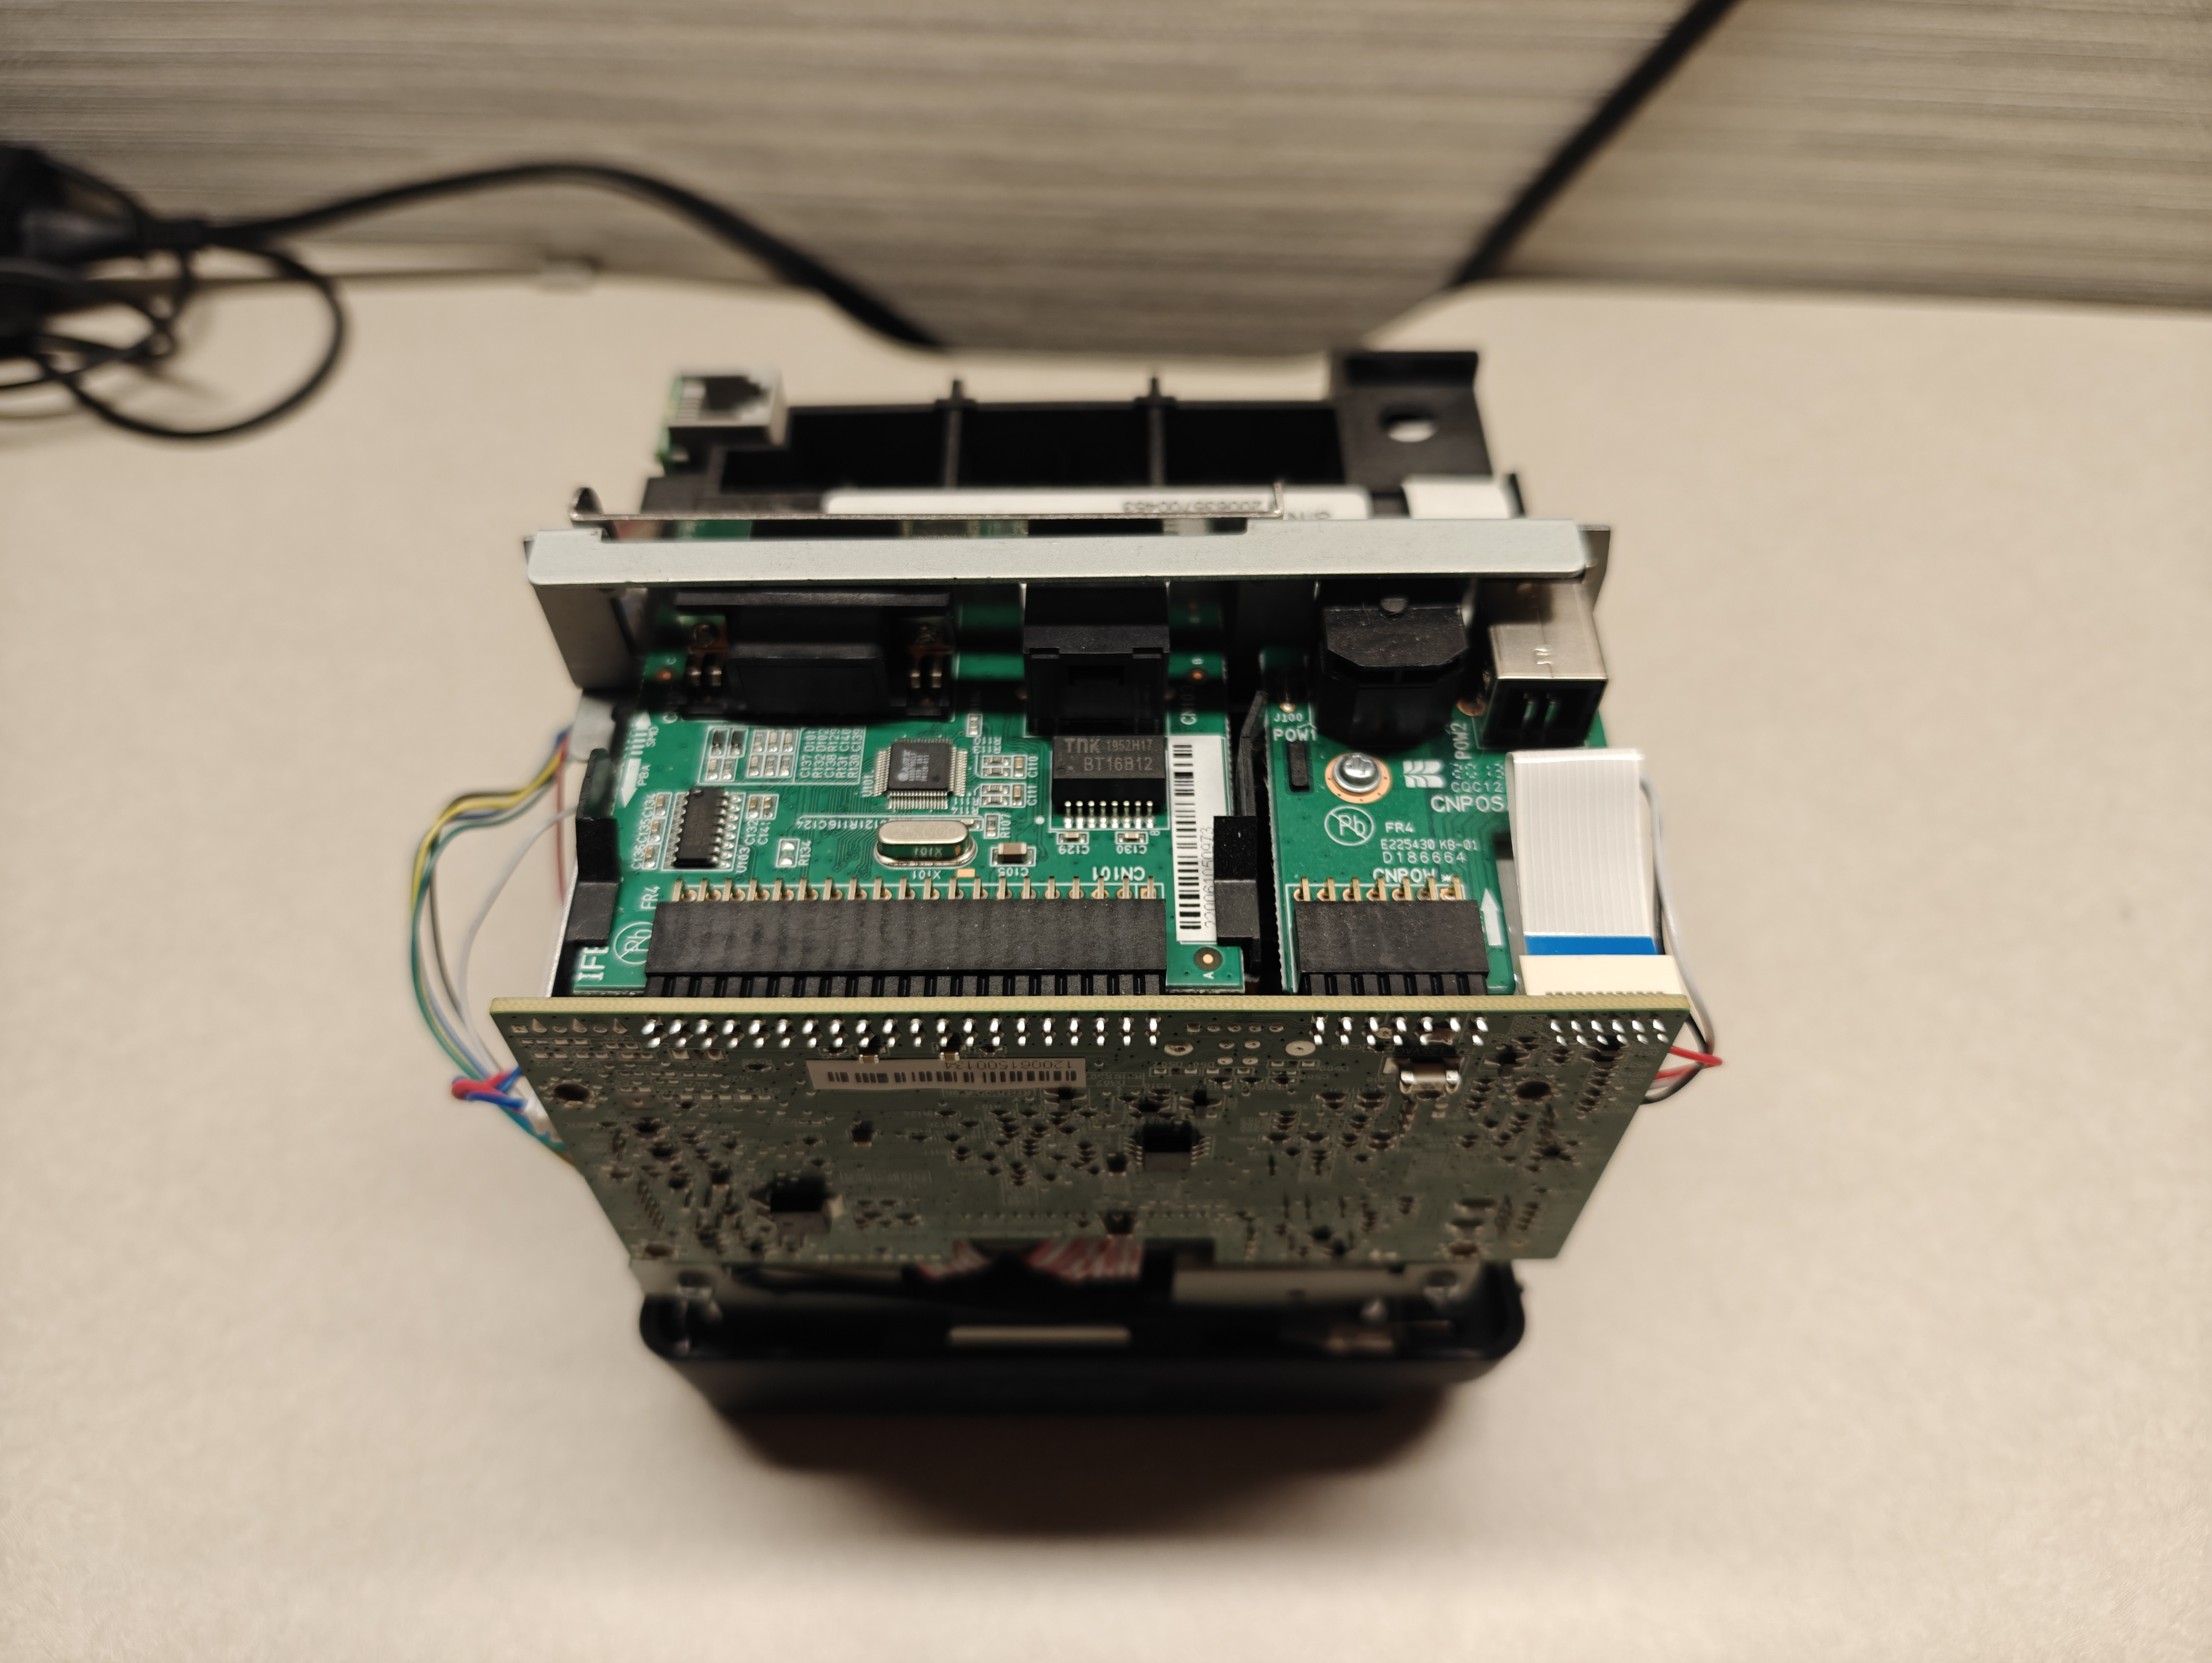
\includegraphics[width=88mm,scale=0.5]
    {Figures/Teardown/IMG20231204171002.jpg}}
    \caption{SNBC BTP-S80 expansion cards}
    \label{fig:snbc_btp_s80_expansion}
\end{figure}

The disassembly is completed after carefully disconnecting each cable, taking note of their respective connectors, and preparing the boards for component identification. There are plenty of components within the device, however, our concern is only the motherboard and two expansion cards. We are only interested in researching the components used for processing and storing data.


\subsection{Identified Components} \label{identifiedcomponents}


% \begin{itemize}
%     \item Walkthrough of documented teardown of the serial printer
% \end{itemize}

Component identification and analysis is divided into two parts. The first being analysis of the motherboard, and the second being the serial expansion card. Analysis of the power delivery and USB type-b expansion card is not necessary since it features no controllers nor any flash to analyze. In some cases, these might still be used for fuzzing and debugging because labeled connectors are provided, however, this can be ignored with most single wire debugging tools (e.g., Jtagulator or Bus Pirate).

\begin{figure}[ht]
    \centering
    {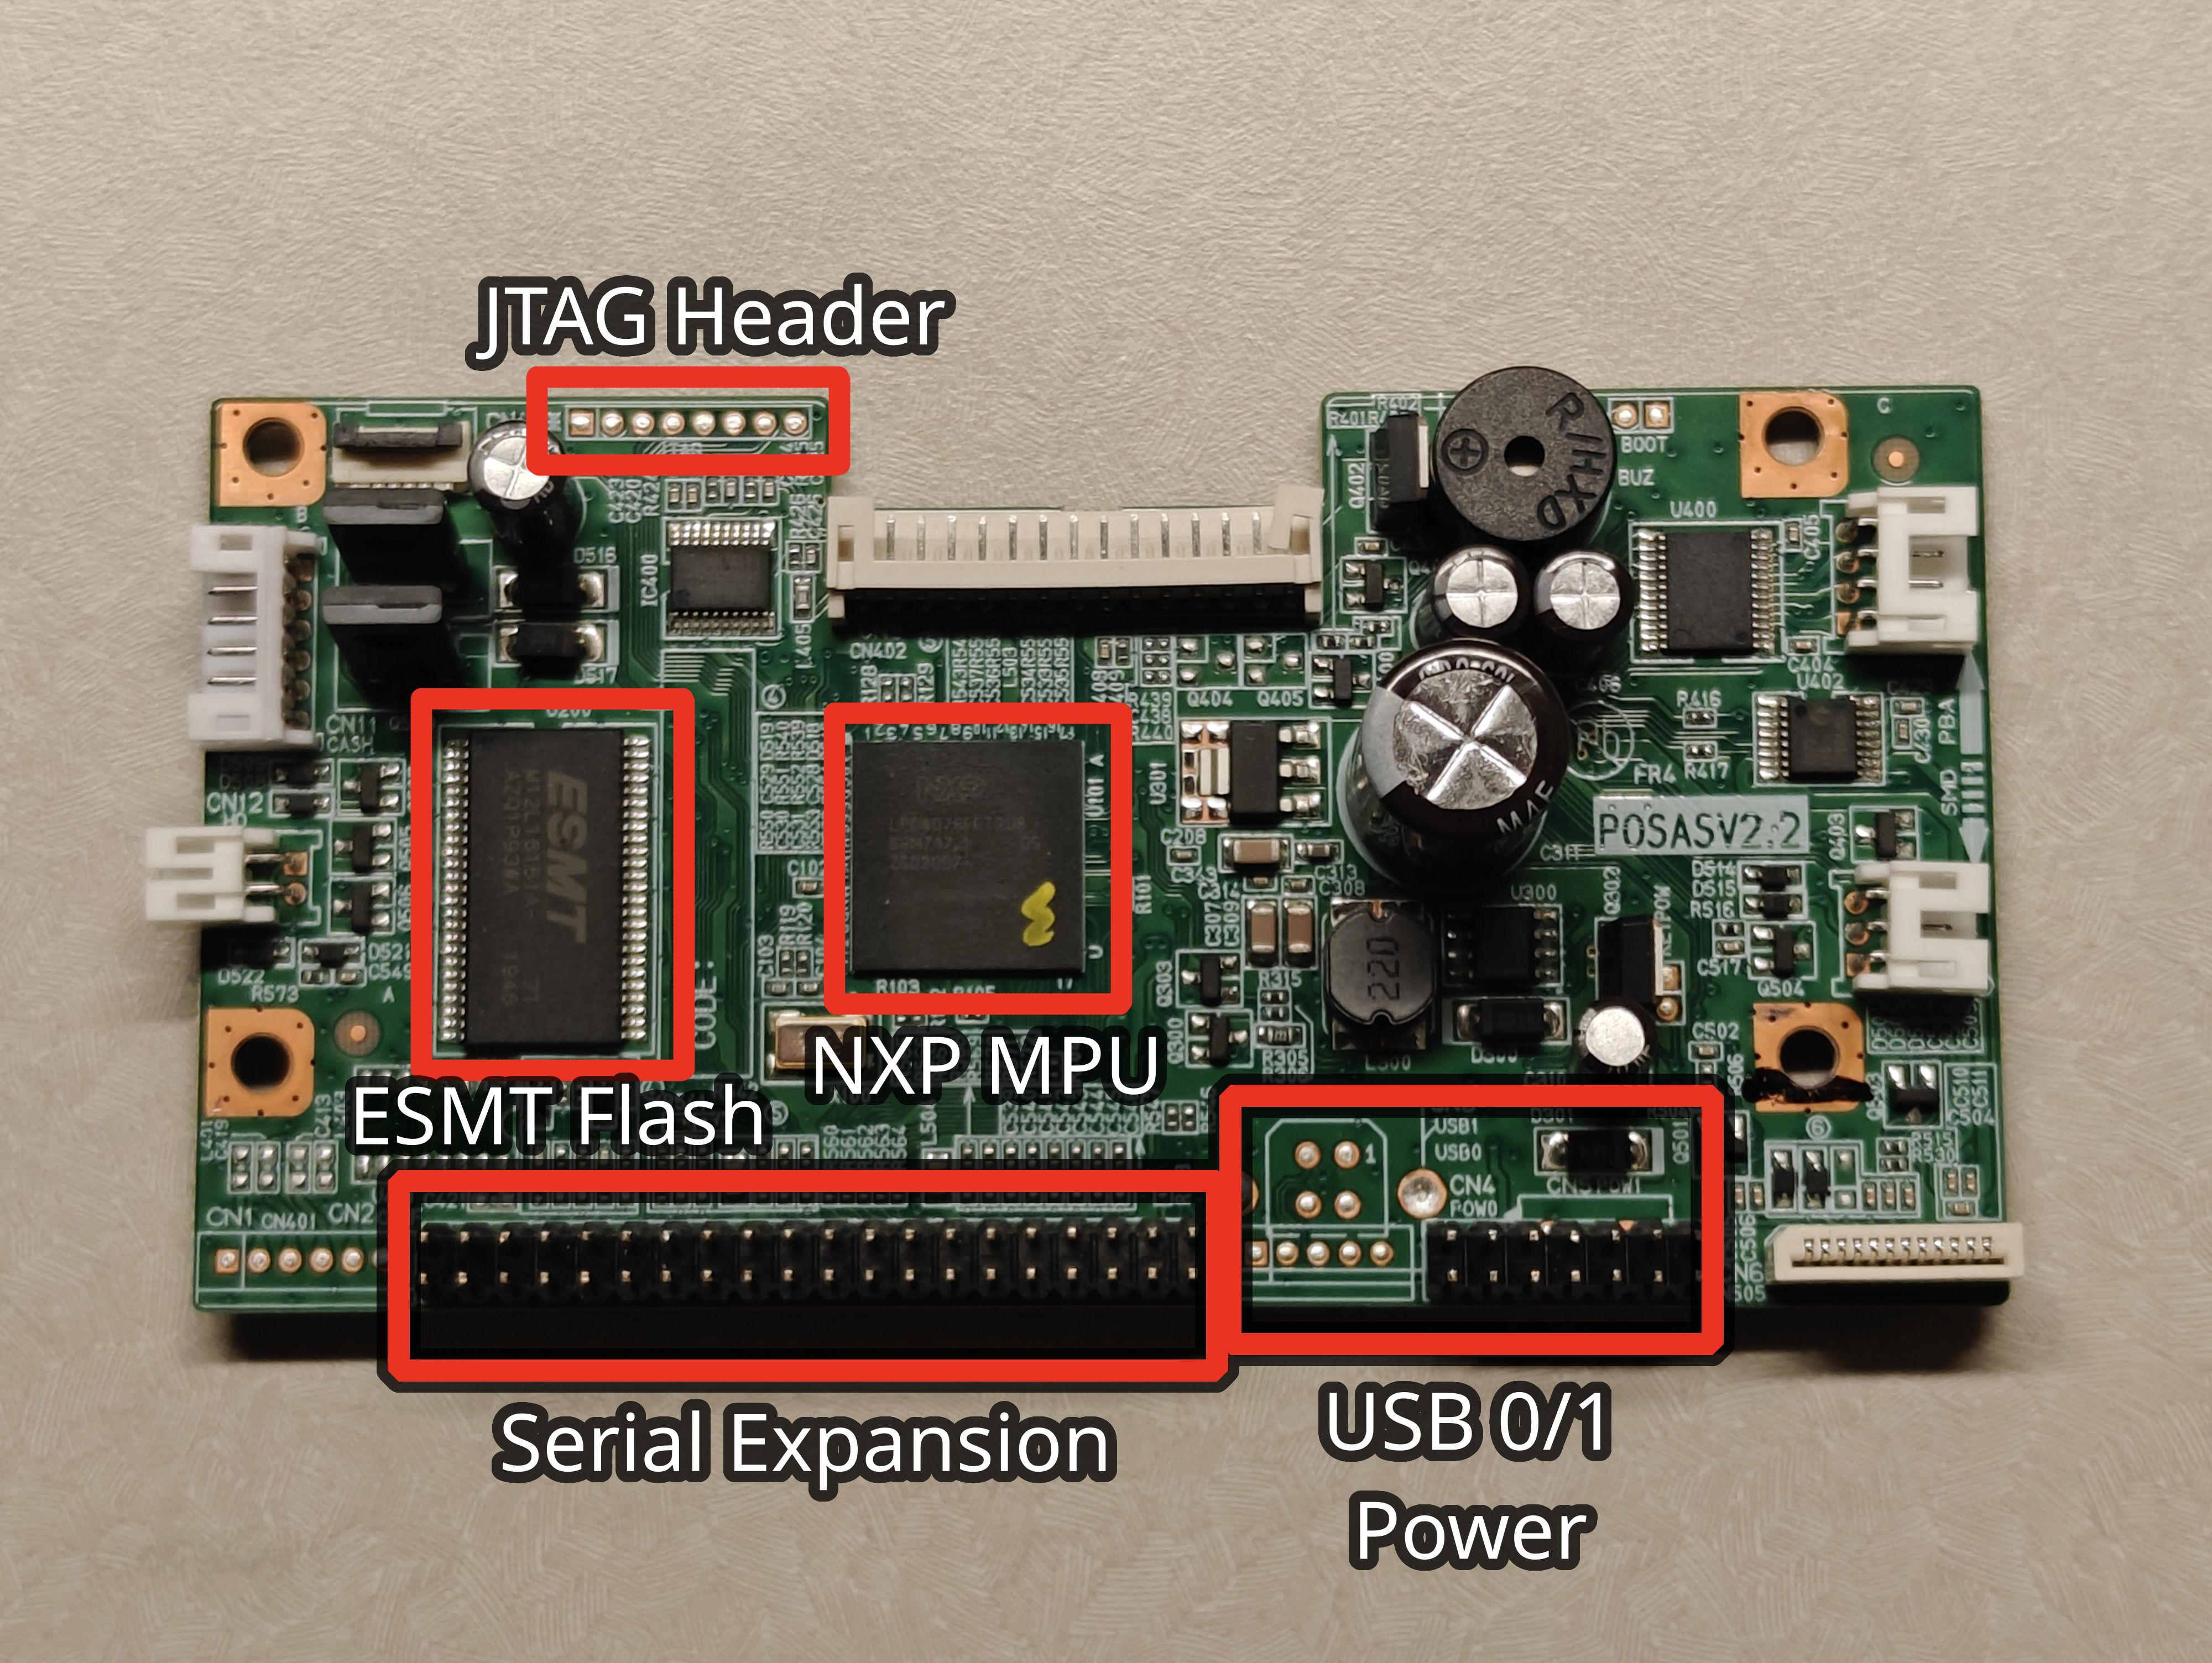
\includegraphics[width=88mm,scale=0.5]
    {Figures/Teardown/IMG20231204171516_annotated.jpg}}
    \caption{Motherboard components}
    \label{fig:snbc_btp_s80_motherboard}
\end{figure}

The list of motherboard components, as shown in Figure \ref{fig:snbc_btp_s80_motherboard}:
\begin{itemize}
    \item NXP 32-bit ARM Cortex-M4 MCU, LPC4078FET208
    \item ESMT DRAM, M12L16161A-7T
\end{itemize}

\begin{figure}[ht]
    \centering
    {\includegraphics[width=88mm,scale=0.5]
    {Figures/Teardown/IMG20231204171204_annotated.jpg}}
    \caption{Expansion card components}
    \label{fig:snbc_btp_s80_expansion_components}
\end{figure}

The list of expansion components, as shown in Figure \ref{fig:snbc_btp_s80_expansion_components}:
\begin{itemize}
    \item SIPEX RS-232 Transceiver, SP2209E
    \item ASIX Ethernet Controller, AX88796C
\end{itemize}

All of these parts can be identified by reading the labeled markings. Typically, there is a manufacturer logo, production date (e.g., YYMM), lot number, and part number. Using this information we cross reference a part database to validate the package of the component (e.g., QFP versus BGA types) and functionality. The records should tell us whether the component is the main processing unit, flash storage, or a micro-controller. Refer to Tables XX for relevant specifications regarding each component. This information aides the firmware analysis section as well as future research.

\begin{table*}
    \centering
    \label{table:LPC4078FET208}%
    \caption{NXP 32-bit ARM Cortex-M4 MCU, LPC4078FET208 \autocite{alldatasheet.comLPC4078FET208DatasheetPDF}}
    \begin{tabular}{|p{4cm}|p{12cm}|}
        \hline\rowcolor{gray!30}
    
        \textbf{Specifications} &  \\
        \hline
    
        Architecture & 32-bit ARM \\
        \hline
    
        Platform & ARM Cortex-M4 \\
        \hline
    
        Frequency & 120-MHz performance \\
        \hline
    
        Memory & 512 kB flash program memory \\
         & 96kB SRAM data memory \\
         & 4032 bytes of EEPROM data memory \\
        \hline

        Features & External Memory Controller (EMC) \\
         & General Purpose DMA Controller \\
         & Quadrature Encoder Interface \\
         & CRC calculation engine \\
         & Code Read Protection (CRP) \\
        \hline
    
        Advanced Comm. Interfaces & UART, SPIFI, I2C, USB/OTG, Ethernet, SSP \\
        \hline
    
        Debug Interfaces & JTAG, SWD \\
        \hline

        Power & Single 3.3V (2.4V to 3.6V) \\
        \hline
    
        Package format & 208-ball, TFBGA208 \\
        \hline
    
    \end{tabular}
\end{table*}

\begin{table*}
    \centering
    \label{table:M12L16161A-7T}%
    \caption{ESMT DRAM, M12L16161A-7T \autocite{alldatasheet.comM12L16161A7TDatasheetPDF}}
    \begin{tabular}{|p{4cm}|p{12cm}|}
      \hline\rowcolor{gray!30}
  
      \textbf{Specifications} &  \\
      \hline
  
      Single power supply operation & 3.3V \\
      \hline
  
      Software Features & CMOS Technology \\
      & Synchronous high data rate DRAM \\
      & LVTTL compatible with multiplexed address \\
      & Burst Read Single-bit Write operation \\
      \hline
  
      Memory architecture & Dual banks operation \\
      & 16,777,216 bits organized as 2 x 524,288 words by 16 bits\\
      \hline
  
      Package format & 50-pin, TSOP \\
      \hline
  
    \end{tabular}
\end{table*}

\begin{table*}
    \centering
    \label{table:SP2209E}%
    \caption{SIPEX High ESD Dual Port RS-232 Transceiver, SP2209E \autocite{alldatasheet.comSP2209EDatasheetPDF}}
    \begin{tabular}{|p{4cm}|p{12cm}|}
      \hline\rowcolor{gray!30}
  
      \textbf{Specifications} &  \\
      \hline
  
      Single power supply operation & 12V \\
      & Operates with +3V or +5V logic as well as standby \\
      \hline

      Comm. Interfaces & Two serial ports, Six drivers, and 10 receivers \\
      & One receiver on each port for active standby \\
      & 460kbps minimum data rate \\
      \hline

      Features & LapLink Compatible \\
      & Low EMI Emissions (EN55022) \\
      & Fast Transient Burst (EFI) Immunity (EN61000-4-2) \\
      & Pin compatible with ADM2209E \\
      \hline
  
      Package format & 38-pin, TSSOP \\
      \hline
  
    \end{tabular}
\end{table*}

\begin{table*}
    \centering
    \label{table:AX88796C}%
    \caption{ASIX Low-Power SPI or Non-PCI Ethernet Controller, AX88796C \autocite{AX88796CPdfAX88796C}}
    \begin{tabular}{|p{4cm}|p{12cm}|}
      \hline\rowcolor{gray!30}

      \textbf{Specifications} &  \\
      \hline
  
      Power & Variable voltage I/O (1.8/2.5/3.3V) \\
      & Programmable driving strength (8/16mA) \\
      \hline

      Software Features & SPI slave interface for CPU w/ SPI master \\
      & Interrupt pin with programmable timer \\
      & IPv4/IPv6 checksum offload engine \\
      & VLAN match filter \\
      & IEEE 802.3/802.3u standards for 10Base-T/100Base-TX \\
      \hline
  
      Memory & 8/16-bit SRAM-like host interface \\
      & Supports Slave-DMA to minimize CPU overhead \\
      & Burst mode read and write access over SRAM-like interface \\
      & Embeds 14KB SRAM packet buffers \\
      & Supports optional EEPROM interface for MAC storage \\
      \hline
   
      Package format & 64-pin, LQFP \\
      \hline
  
    \end{tabular}
\end{table*}


\subsection{Technical Resources} \label{technicalresources}

% List and describe datasheets and  source - AllDataSheets.com

% \textbf{Outline}
% $\downarrow$

% \begin{itemize}
%     \item List datasheets and where they were sourced
%     \item Explanation of which sites/resources and why
% \end{itemize}

All technical data and specifications sheets were procured through AllDataSheet or FindChips \autocite{ALLDATASHEETCOMElectronic,FindchipsElectronicPart}. There is a litany of other sources that can be used, however, these are the ones used by the researcher. There are no empirical reasons for using these sources instead of others, it was purely motivated by personal preference. Regardless of whichever datasheet aggregator is used, it should not harm replicability of the research.

\subsection{Firmware Analysis} \label{firmwareanalysis}

% \textbf{Outline}
% $\downarrow$

% \begin{itemize}
%     \item List bootloader information
%     \item Details about recovered memory regions (e.g., addr ranges, size, perms)
%     \item Known libraries
% \end{itemize}

As shown in Section \ref{hardwareassessment} Hardware Assessment, we can determine the correct pin layout for interfacing with the debug headers using the manufacturer datasheet. Whether or not this process is successful largely depends on the type of component packaging. In the previous example where we demonstrated reading the datasheet in relation to the pin diagram, it was possible to attach a debugger to the interface without a header prepared by the manufacturer on the device PCB. This is not possible for the SNBC BTP-S80.

Figure \ref{fig:snbc_btp_s80_motherboard} and the corresponding datasheet, shows us that the MPU uses a 208-ball thin and fine ball grid array (TFBGA) package. Unless we used a process called decapsulation or delamination it is not possible to access these pins without risking damage to the device \autocite{sanchezlopezContributionStudyElectronic2015}. The manufacturers of the BTP-S80 were kind enough to provide a JTAG debug header, as shown and labeled in Figure \ref{fig:snbc_btp_s80_motherboard}.

However, the exact pin layout is not provided. This can easily be verified manually via a multimeter and logic analyzer while referencing the manufacturer documentation. The process can be time consuming for those unfamiliar and it is recommended to use a tool such as the Jtagulator \autocite{JTAGulator2023} for enumerating the correct configuration.

With the ground and voltage reference pins validated, the researcher can connect up to 24 channels or pins. The tool will then check every permutation of the channels until an available header is identified. Using this information, we can continue with the Jtagulator or another USB debugger to continue our investigation.


\section{Conclusion}

% \textbf{Outline}
% $\downarrow$

% \begin{itemize}
%     \item Reiterate the introduction, research questions, and how the results of the research answered those questions.
%     \item Provide supporting statements for future research and highlight areas that were loosely documented/known and would have been solid preliminary research.
%     \item Can these devices be extended? Research questions, yes/no...
% \end{itemize}

% \begin{itemize}
%     \item Summary of physical protections (e.g., too much information silkscreened on PCB)
%     \item List hardware protections (e.g., did manufacturer block debug access, are memory regions locked)
%     \item Discuss software protections (e.g., access to bootloader, identifiable CVEs/CWEs, attributable libraries/functions)
% \end{itemize}

In conclusion, the researcher was able to demonstrate four of the five objectives for the research. We identified baseline of the hardware and operating system used by the serial printer. We identified the specific version of the operating system, any supporting libraries as well as their versions (i.e., RT-Thread RTOS). We were also able to clearly demonstrate that the manufacturers have enabled minimal security protections despite the hardware supporting them; which, is especially worth noting because the operating system itself has minimal protections for isolating memory across processes other than CRC checksums. It is also possible, as demonstrated, to be able to reflash the memory utilizing the MCU hardware debug interfaces.

Due to underestimating the time needed for delivery of the additional devices for the proposed sample population, only one device was assessed. Although the SNBC BTP-S80 is a fairly common serial printer used across financial sectors as well as industrial control, the research would have been better represented with the cross-examination against several other devices. Lastly, another goal of the research was to use the gathered data to support the proposal of future research into a design artifact for implementing BadUSB-like concepts on peripheral serial devices. 

% Add the references
\printbibliography

\vspace{12pt}

\end{document}
